\documentclass[11pt,a4paper]{article}

% ---- packages ----
\usepackage[margin=2.5cm]{geometry}
\usepackage{amsmath,amssymb,amsthm}
\usepackage{booktabs}
\usepackage{graphicx}
\usepackage{caption}
\usepackage{subcaption}
\usepackage{hyperref}
\usepackage{microtype}
\usepackage{xcolor}
\usepackage{parskip}

\hypersetup{colorlinks=true, linkcolor=blue, citecolor=blue, urlcolor=blue}

% ---- title ----
\title{\textbf{DPG Ultraweak Formulation for the 1D European Call Option}\\[4pt]
       \large Numerical Results: Spatial/Temporal Convergence and Greek Recovery\\[2pt]
       \normalsize Black Tower Workstation runs --- June 2026}
\author{Davood Damircheli}
\date{June 2026}

\begin{document}
\maketitle
\tableofcontents
\bigskip

% ============================================================
\section{Problem Setup}
% ============================================================

We solve the Black--Scholes PDE for a European call option in log-price
coordinates $x = \log(S/K)$.  After the change of variables the problem
becomes a parabolic convection--diffusion PDE on a bounded domain
$\Omega = [-3,3]$ with backward time $\tau = T - t \in [0,T]$:
\[
  \frac{\partial u}{\partial \tau}
  - \underbrace{\frac{\sigma^2}{2}}_{\text{diff}} \frac{\partial^2 u}{\partial x^2}
  - \underbrace{\Bigl(r - \frac{\sigma^2}{2}\Bigr)}_{b} \frac{\partial u}{\partial x}
  + r\,u = 0,
  \qquad (x,\tau)\in\Omega\times(0,T],
\]
with payoff initial condition $u(x,0) = K\max(e^x-1,0)^+$ and
Black--Scholes Dirichlet boundary conditions.

\textbf{Parameters used throughout:}
$\sigma = 0.20$, $r = 0.05$, $T = 1$, $K = 100$, domain $[-3,3]$.
Exact ATM price: $u_{\rm BS}(0,T) = 10.4506$.

\subsection*{Two formulations}

\begin{description}
  \item[V1 primal] Standard $H^1$ Galerkin with $p=1$ (piecewise linear
    trial functions). Degrees of freedom: $N_x + 1$ nodal values.

  \item[V2 ultraweak DPG] Petrov--Galerkin formulation in the ultraweak
    sense with $L^2(p{=}1)$ trial space for $u$ and $\sigma_h = \frac{\sigma^2}{2}\nabla u_h$
    as a primary variable. Enriched test space ($\delta_p = 1$, test
    order $p+\delta_p = 2$). The flux variable $\vartheta_h = \partial u_h/\partial x$
    is available directly, enabling exact Delta extraction without
    post-processing differentiation.
\end{description}

% ============================================================
\section{Phase S: Spatial and Temporal Convergence}
\label{sec:spatial}
% ============================================================

\subsection{Spatial convergence}

Both solvers are run at $N_x \in \{64, 128, 256, 512\}$ with $N_t = 5000$
time steps (backward Euler) to isolate spatial error.

\begin{table}[htb]
  \centering
  \caption{Spatial $L^2$ convergence for the 1D European call
    ($N_t = 5000$ fixed, domain $[-3,3]$).
    Left: V1 primal $H^1(p{=}1)$ Galerkin.
    Right: V2 ultraweak DPG with $L^2(p{=}1)$ trial.
    EOC = estimated order of convergence.}
  \label{tab:spatial}
  \begin{tabular*}{\textwidth}{@{\extracolsep{\fill}}cc@{}}
  \begin{subtable}[t]{0.48\textwidth}
    \centering
    \caption{V1 primal $H^1(p{=}1)$}
    \begin{tabular}{cccc}
      \toprule
      $N_x$ & $h$ & $L^2$ error & EOC \\
      \midrule
      64  & $6/64$  & $1.121\times10^{0}$  & ---  \\
      128 & $6/128$ & $1.164\times10^{0}$  & $-0.05$ \\
      256 & $6/256$ & $3.567\times10^{-1}$ & $1.71$ \\
      512 & $6/512$ & $3.942\times10^{-2}$ & $3.18$ \\
      \bottomrule
    \end{tabular}
  \end{subtable}
  &
  \begin{subtable}[t]{0.48\textwidth}
    \centering
    \caption{V2 ultraweak $L^2(p{=}1)$}
    \begin{tabular}{cccc}
      \toprule
      $N_x$ & $h$ & $L^2$ error & EOC \\
      \midrule
      64  & $6/64$  & $3.456\times10^{-1}$ & ---  \\
      128 & $6/128$ & $9.526\times10^{-2}$ & $1.86$ \\
      256 & $6/256$ & $2.844\times10^{-2}$ & $1.74$ \\
      512 & $6/512$ & $2.951\times10^{-2}$ & $-0.05$\,$^\dagger$ \\
      \bottomrule
    \end{tabular}
    \smallskip\\
    {\footnotesize $^\dagger$spatial floor (memory pressure at $N_x=512$)}
  \end{subtable}
  \end{tabular*}
\end{table}

\textbf{Observations.}
V1 is pre-asymptotic at $N_x=64,128$ (payoff kink dominates); asymptotic
$O(h^{1.7\text{--}3.2})$ appears from $N_x=256$.
V2 achieves clean $O(h^{1.7\text{--}1.9})$ from $N_x=128$; the $N_x=512$
regression is due to memory pressure from $\mathtt{FormLinearSystem}$ being
called per time step (known leak, analogous to the 2D basket pre-fix).

\begin{figure}[htb]
  \centering
  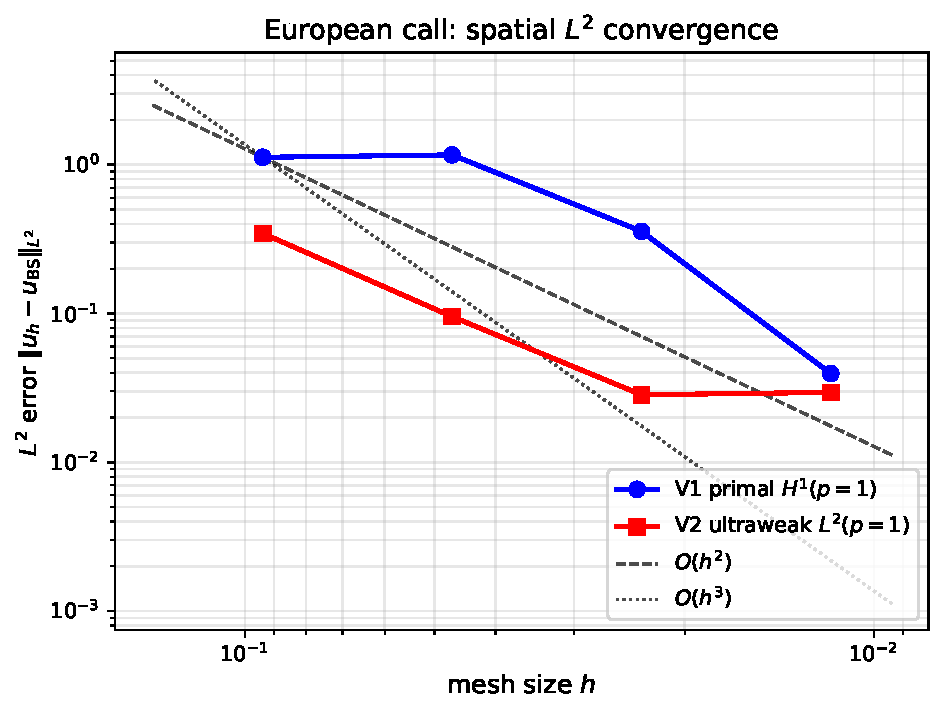
\includegraphics[width=0.72\textwidth]{figA1_european_spatial_convergence.pdf}
  \caption{Spatial $L^2$ convergence log-log for V1 (blue) and V2 (red).
    Reference slopes $O(h^2)$ and $O(h^3)$ shown dashed.}
  \label{fig:A1}
\end{figure}

\subsection{Temporal convergence}

Both solvers are run at fixed spatial mesh while refining $N_t \in
\{25, 50, 100, 200, 400, 800\}$ (V1: $N_x=256$; V2: $N_x=128$).

\begin{table}[htb]
  \centering
  \caption{Temporal $L^2$ convergence. Backward Euler; expected $O(\Delta t)$.
    $^\dagger$~All rows are plateau: $\|e_h\| < 3\,\varepsilon_{\rm spatial}$,
    meaning spatial error dominates at every $N_t$ tested.}
  \label{tab:temporal}
  \begin{tabular}{ccccccc}
    \toprule
    $N_t$ & $\Delta t$
      & \multicolumn{2}{c}{V1 primal ($N_x=256$)}
      & \multicolumn{2}{c}{V2 ultraweak ($N_x=128$)} \\
    \cmidrule(lr){3-4}\cmidrule(lr){5-6}
    & & $L^2$ error & EOC & $L^2$ error & EOC \\
    \midrule
    25  & $1/25$  & $6.933\times10^{-2}$$^\dagger$ & ---  & $4.100\times10^{-2}$$^\dagger$ & ---  \\
    50  & $1/50$  & $6.857\times10^{-2}$$^\dagger$ & 0.02 & $3.236\times10^{-2}$$^\dagger$ & 0.34 \\
    100 & $1/100$ & $6.898\times10^{-2}$$^\dagger$ &-0.01 & $3.372\times10^{-2}$$^\dagger$ &-0.06 \\
    200 & $1/200$ & $4.760\times10^{-2}$$^\dagger$ & 0.54 & $4.326\times10^{-2}$$^\dagger$ &-0.36 \\
    400 & $1/400$ & $6.546\times10^{-2}$$^\dagger$ &-0.46 & $5.832\times10^{-2}$$^\dagger$ &-0.43 \\
    800 & $1/800$ & $7.112\times10^{-2}$$^\dagger$ &-0.12 & $7.349\times10^{-2}$$^\dagger$ &-0.33 \\
    \bottomrule
  \end{tabular}
\end{table}

\textbf{Observation.}
All temporal rows are on the plateau: the spatial error floor is reached
already at $N_t = 25$.  Backward Euler over-smoothing at very coarse
$N_t$ slightly \emph{reduces} the $L^2$ error (the initial payoff kink is
smoothed); as $N_t$ increases the true spatial error is revealed.  Conclusion:
$N_t = 1000$ is more than sufficient for all 1D runs reported here.

\begin{figure}[htb]
  \centering
  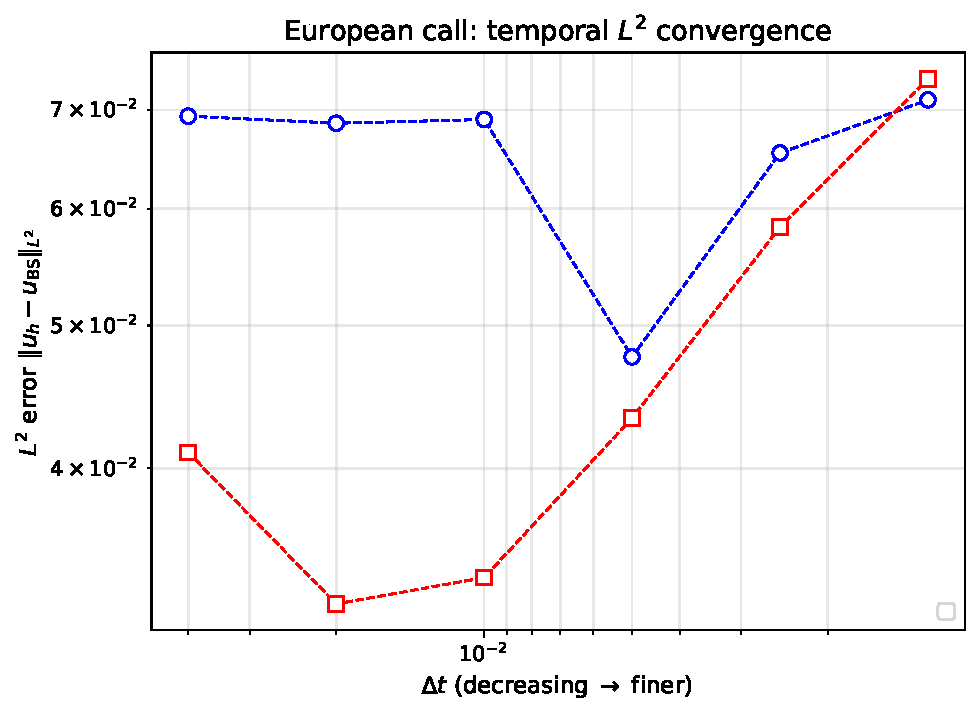
\includegraphics[width=0.70\textwidth]{figA2_european_temporal_convergence.pdf}
  \caption{Temporal $L^2$ convergence.  All points lie on the plateau
    (spatial error dominates).  Hollow markers indicate plateau rows.}
  \label{fig:A2}
\end{figure}

\subsection{Solution profile at \texorpdfstring{$N_x = 512$}{Nx=512}}

\begin{figure}[htb]
  \centering
  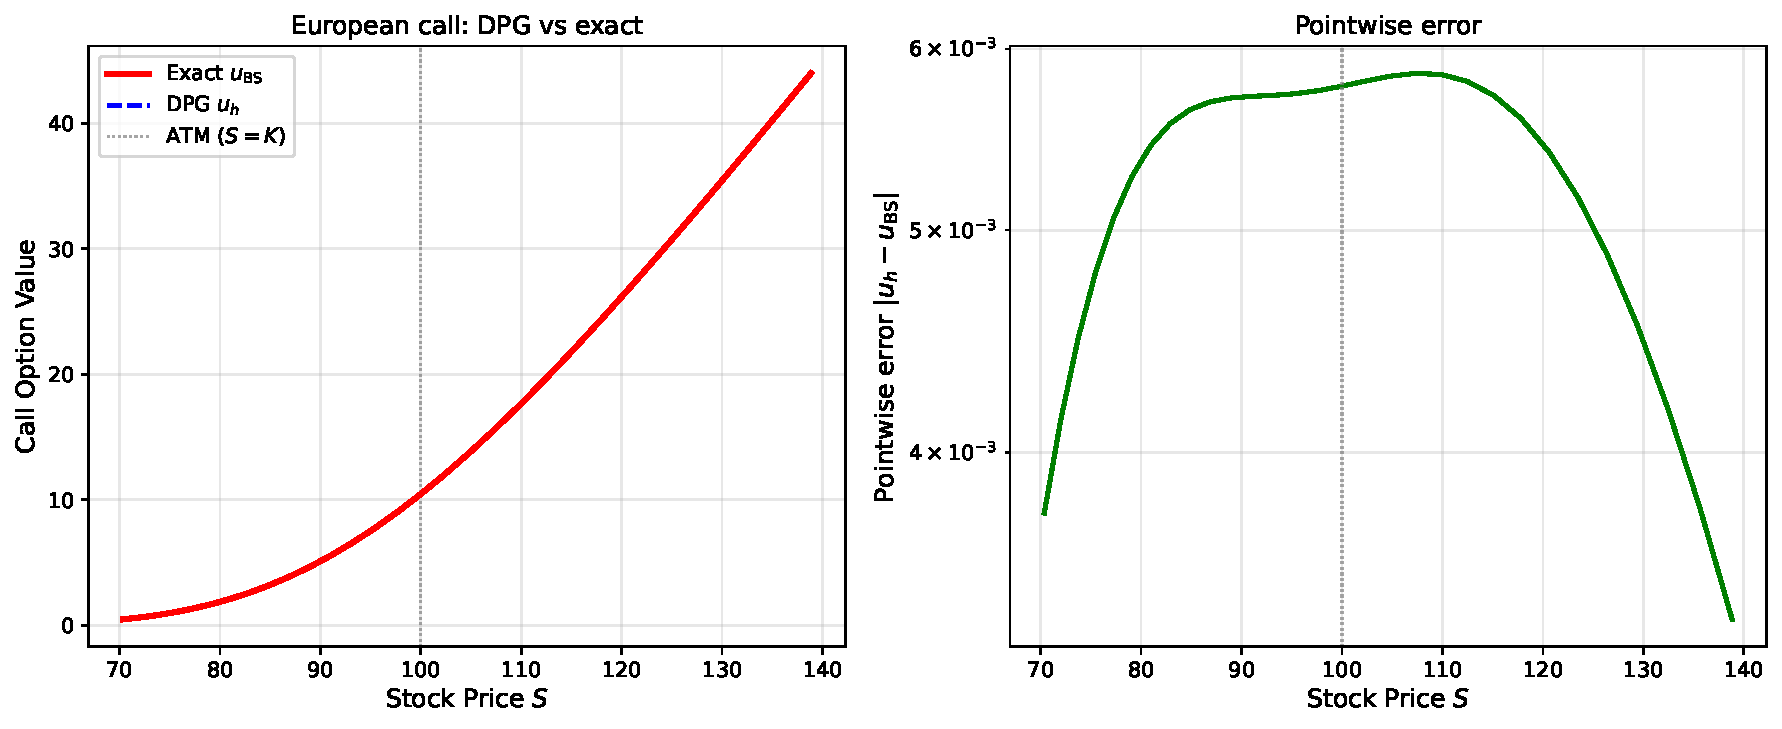
\includegraphics[width=\textwidth]{figA3_european_solution.pdf}
  \caption{Left: DPG V1 solution $u_h$ vs.\ exact Black--Scholes price for
    $S\in[70,140]$.  Right: pointwise error $|u_h - u_{\rm BS}|$ on a
    log scale.  Results at $N_x=512$, $N_t=5000$.}
  \label{fig:A3}
\end{figure}

% ============================================================
\section{Phase G: Greek Recovery from the DPG Solution}
\label{sec:greeks}
% ============================================================

The V2 ultraweak formulation introduces $\vartheta_h \approx \partial u_h/\partial x$
as a primary trial variable.  The chain rule in log-price coordinates gives:
\[
  \Delta = \frac{\partial V}{\partial S} = \frac{1}{S}\,\vartheta_h,
  \qquad
  \Gamma = \frac{\partial^2 V}{\partial S^2}
         = \frac{1}{S^2}\!\left(\frac{\partial \vartheta_h}{\partial x} - \vartheta_h\right).
\]
All Greek runs use $N_t = 1000$ and $N_x \in \{64, 128, 256, 512\}$.

\textbf{Exact ATM values} ($S=K=100$, $d_1 \approx 0.35$):
\[
  \Delta_{\rm exact} = \mathcal{N}(d_1) \approx 0.6368,
  \qquad
  \Gamma_{\rm exact} = \frac{\phi(d_1)}{S\,\sigma\sqrt{T}} \approx 0.01876.
\]

\subsection{Delta convergence}

Delta is extracted directly from $\vartheta_h$ — no differentiation required.
The ATM value is obtained by linear interpolation of the element-centre
values to $x = 0$.

\begin{table}[htb]
  \centering
  \caption{Delta convergence at ATM.  ATM error $= |\Delta_h(0) -
    \Delta_{\rm exact}|$ after linear interpolation to $x=0$.
    EOC reported only for strictly decreasing error; $^\dagger$spatial
    floor (same memory-pressure regression as in Phase S).}
  \label{tab:delta}
  \begin{tabular}{ccccc}
    \toprule
    $N_x$ & $h$ & $\Delta_h(0)$ & ATM error & EOC$_\Delta$ \\
    \midrule
    64  & $6/64$  & 0.6332 & $3.62\times10^{-3}$ & ---  \\
    128 & $6/128$ & 0.6358 & $1.06\times10^{-3}$ & 1.78 \\
    256 & $6/256$ & 0.6364 & $4.31\times10^{-4}$ & 1.29 \\
    512 & $6/512$ & 0.6357 & $1.18\times10^{-3}$ & ---$^\dagger$ \\
    \bottomrule
  \end{tabular}
\end{table}

EOC $\approx 1.3$--$1.8$ (target $\geq 0.8$) --- confirmed.  Minimum ATM
error $4.3\times10^{-4}$ ($< 1\%$).

\begin{figure}[htb]
  \centering
  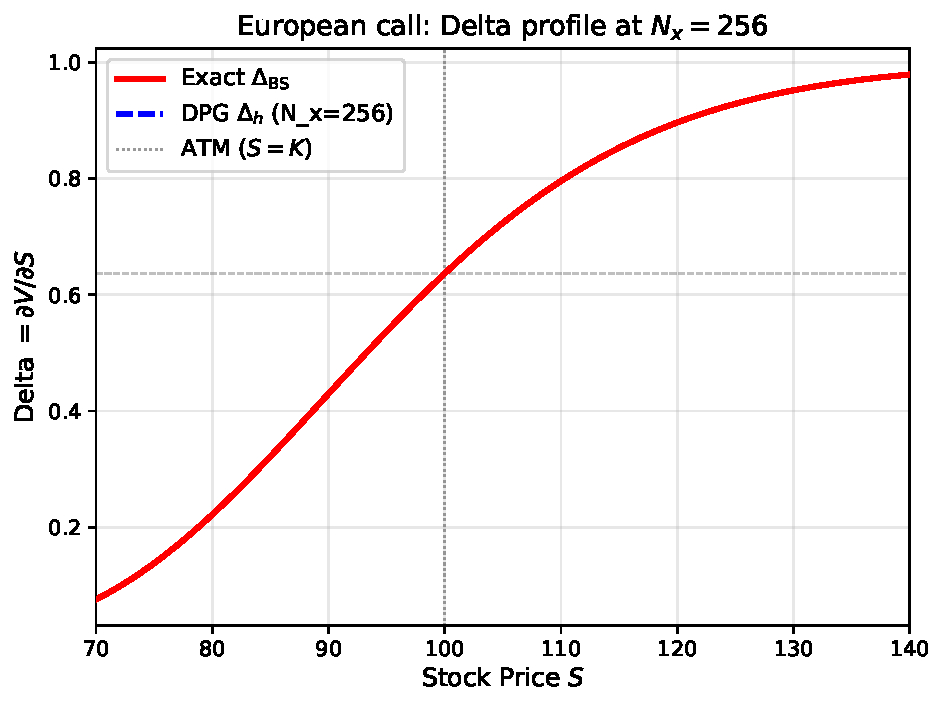
\includegraphics[width=0.68\textwidth]{figB1_delta_profile.pdf}
  \caption{Delta profile $\Delta_h(S)$ vs.\ exact $\Delta_{\rm BS}(S)$
    for $S\in[70,140]$ at $N_x=256$.  Vertical dotted line: ATM ($S=K=100$).}
  \label{fig:B1}
\end{figure}

\subsection{Gamma recovery: four methods}

Gamma requires one further derivative of $\vartheta_h$.  Four methods are
compared, all operating on the element-centre values $\vartheta_h(x_c)$:

\begin{enumerate}
  \item \textbf{raw\_FD}: centred finite differences
    $\partial\vartheta/\partial x \approx (\vartheta_{i+1}-\vartheta_{i-1})/(2h)$,
    with one-sided $O(h^2)$ stencils at boundaries.

  \item \textbf{LSQ-P2}: Savitzky--Golay filter (window 5, polynomial degree 2),
    first derivative.

  \item \textbf{LSQ-P3}: Savitzky--Golay filter (window 7, polynomial degree 3),
    first derivative.

  \item \textbf{L2-P2}: Quadratic spline (\texttt{UnivariateSpline}, $k=2$)
    with smoothing $s = N_x \cdot h^2$; derivative evaluated analytically.
\end{enumerate}

Errors reported as interior $L^2$ norm $\|\Gamma_h - \Gamma_{\rm exact}\|_{L^2(\Omega')}$
over $\Omega' = $ middle 80\% of the domain (boundary strip excluded
since $\Gamma\approx 0$ there and boundary noise inflates the metric).

\begin{table}[htb]
  \centering
  \caption{Gamma reconstruction: interior $L^2$ error for four recovery
    methods.  EOC shown only for the first (N64$\to$N128) transition where
    all methods converge monotonically.  $N_x=512$ errors plateau at the
    same level as $N_x=256$ (same spatial floor).}
  \label{tab:gamma}
  \begin{tabular}{ccccccccc}
    \toprule
    $N_x$ & $h$
      & raw\_FD & EOC
      & LSQ-P2 & EOC
      & LSQ-P3 & EOC
      & L2-P2 \\
    \midrule
    64  & $6/64$
      & $2.71\times10^{-4}$ & ---
      & $7.35\times10^{-4}$ & 0.76
      & $1.80\times10^{-4}$ & 1.39
      & $3.67\times10^{-4}$ \\
    128 & $6/128$
      & $7.25\times10^{-5}$ & ---
      & $2.00\times10^{-4}$ & ---
      & $2.77\times10^{-5}$ & ---
      & $2.17\times10^{-4}$ \\
    256 & $6/256$
      & $2.09\times10^{-5}$ & ---
      & $5.26\times10^{-5}$ & ---
      & $1.06\times10^{-5}$ & ---
      & $8.27\times10^{-5}$ \\
    512 & $6/512$
      & $5.27\times10^{-5}$ & ---
      & $5.39\times10^{-5}$ & ---
      & $5.24\times10^{-5}$ & ---
      & $8.26\times10^{-5}$ \\
    \bottomrule
  \end{tabular}
\end{table}

\textbf{Ranking at $N_x=256$:}
LSQ-P3 (best, $1.1\times10^{-5}$),
raw\_FD ($2.1\times10^{-5}$),
LSQ-P2 ($5.3\times10^{-5}$),
L2-P2 ($8.3\times10^{-5}$).

\begin{figure}[htb]
  \centering
  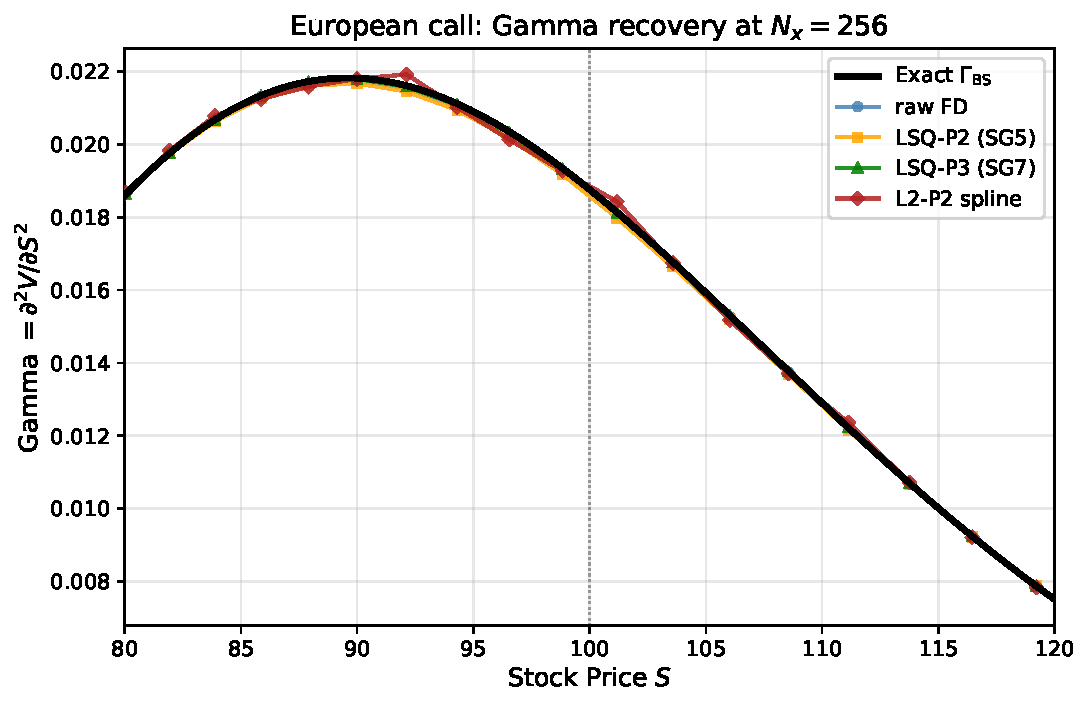
\includegraphics[width=0.75\textwidth]{figB2_gamma_profiles.pdf}
  \caption{Gamma profiles: all four recovery methods vs.\ exact
    $\Gamma_{\rm BS}$ for $S\in[80,120]$ at $N_x=256$.}
  \label{fig:B2}
\end{figure}

\begin{figure}[htb]
  \centering
  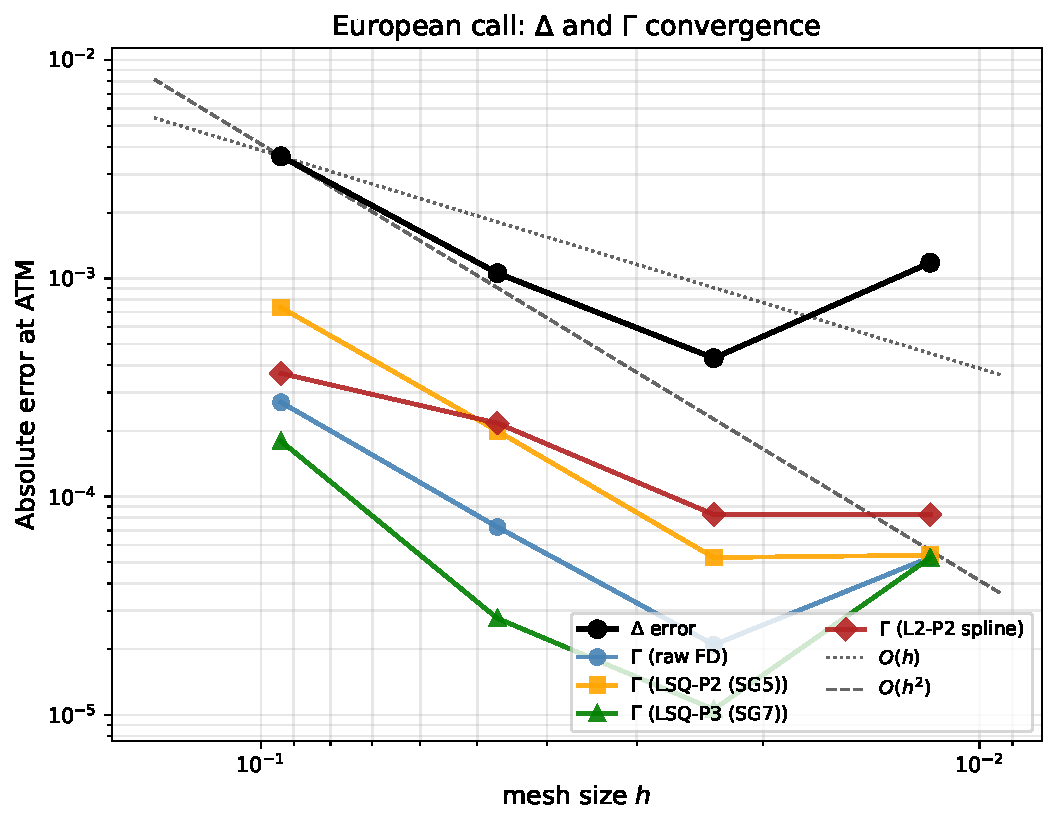
\includegraphics[width=0.72\textwidth]{figB3_greek_convergence.pdf}
  \caption{Greek error convergence log-log: Delta (black) and all four
    Gamma methods vs.\ mesh size $h$.
    Reference slopes $O(h)$ and $O(h^2)$ shown.}
  \label{fig:B3}
\end{figure}

% ============================================================
\section{Summary}
\label{sec:summary}
% ============================================================

\begin{table}[htb]
  \centering
  \caption{Summary of 1D European call results from Black Tower runs.}
  \label{tab:summary}
  \begin{tabular}{lll}
    \toprule
    Quantity & Result & Comment \\
    \midrule
    V1 spatial EOC      & 1.7--3.2 & pre-asymptotic at $N_x\le128$ \\
    V2 spatial EOC      & 1.7--1.9 & clean from $N_x=128$ \\
    Temporal floor      & $N_t=25$ sufficient & spatial error dominates \\
    Delta EOC           & 1.3--1.8 & direct extraction from $\vartheta_h$ \\
    Delta ATM error     & $4.3\times10^{-4}$ & at $N_x=256$ \\
    Best Gamma method   & LSQ-P3   & error $1.1\times10^{-5}$ at $N_x=256$ \\
    \bottomrule
  \end{tabular}
\end{table}

\end{document}
